\documentclass[submit,techrep,noauthor]{ipsj}

\usepackage{amsmath,amssymb,amsfonts}
\usepackage{cite}
\usepackage[japanese]{babel}
\usepackage[scaled]{beramono}
\usepackage{booktabs}
\usepackage{caption}
\usepackage[T1]{fontenc}
\usepackage[dvipdfmx]{graphicx}
\usepackage[utf8]{inputenc}
\usepackage{listings}
\usepackage[all,warning]{onlyamsmath}
\usepackage{siunitx}
\usepackage[subrefformat=parens]{subcaption}
\usepackage{url}

\begin{document}

\title{ベクトル型スーパーコンピュータ「AOBA-S」の性能評価}

\etitle{Performance Evaluation of a Vector Supercomputer ``AOBA-S''}

\affiliate{CSC}{東北大学サイバーサイエンスセンター}
\affiliate{NEC}{日本電気株式会社}
\affiliate{TU}{東北大学大学院情報科学研究科}
\affiliate{TDU}{東京電機大学}

\author{高橋 慧智}{Keichi Takahashi}{CSC,TU}[keichi@tohoku.ac.jp]
\author{藤本 壮也}{Soya Fujimoto}{NEC}[s-fujimoto@nec.com]
\author{長瀬 悟}{Satoru Nagarase}{NEC}[s.nagase@nec.com]
\author{磯部 洋子}{Yoko Isobe}{NEC}[y-isobe-pi@nec.com]
\author{下村 陽一}{Yoichi Shimomura}{CSC}[shimomura32@tohoku.ac.jp]
\author{江川 隆輔}{Ryusuke Egawa}{TDU}[egawa@mail.dendai.ac.jp]
\author{滝沢 寛之}{Hiroyuki Takizawa}{CSC,TU}[takizawa@tohoku.ac.jp]

\begin{abstract}
東北大学サイバーサイエンスセンターは,2023年8月よりベクトル型スーパーコンピュータ「AOBA-S」の運用を
開始した.AOBA-Sは第3世代ベクトルエンジン (VE30) をノードあたり8基搭載した計504ノードから構成され,
理論演算性能は21.05\,PFLOP/s,メモリ帯域幅は9.97\,PB/sに達する世界最大規模のベクトル型
スーパーコンピュータである.本稿ではAOBA-Sの設計を概説し,運用開始に先駆けて実施したAOBA-Sの
初期性能評価の結果について報告する.
\end{abstract}

\begin{eabstract}
Cyberscience Center, Tohoku University has started the operation of a new vector supercomputer 
``AOBA-S'' in August 2023. AOBA-S comprises 504 compute nodes each equipped with eight
third-generation Vector Engine (VE30) cards. The peak compute performance and memory bandwidth of
AOBA-S reach 21.05\,PFLOP/s and 9.97\,PB/s, respectively, making it the world's largest vector
supercomputer as of writing this paper. In this paper, we describe the basic design of AOBA-S and
report the results of the initial performance evaluation that we have conducted prior to the
operation start of AOBA-S.
\end{eabstract}

\maketitle

\section{はじめに}

東北大学サイバーサイエンスセンター (以下本センター) では,1986年に高性能計算センターとして活動を
開始して以来,SX-1 (NEC製,0.57\,GFLOP/s) から一貫して,主力計算システムとして
ベクトル型スーパーコンピュータを導入し,最先端の学術研究を強力に支援,推進してきた.
本センターは全国の大学等の研究者が学術研究のために利用する全国共同利用施設であると同時に,
全国の情報基盤センター群と連携した学際大規模情報基盤共同利用・共同研究拠点 (JHPCN) の構成拠点である.
また,「富岳」を中核とする全国の計算機資源を連携した革新的ハイパフォーマンス・コンピューティング・
インフラ (HPCI) の構成機関でもあり、共同研究活動を推進する拠点となっている.

このような背景の下,本センターでは2020年10月にベクトル型スーパーコンピュータ「AOBA-A」および
スカラ型並列コンピュータ「AOBA-B」を導入し,高速で大規模な計算処理環境を提供してきた.
両サブシステムの利用率は常に高く,計算需要が処理能力を超える状況が続いてきた.そこで,
次期スーパーコンピュータ「AOBA-S」の構想・設計を進めつつ,
2022年10月にはクラウド上システムAOBA-Cによって処理能力の一時的な増強を実施した.
AOBA-Sの入札公示は2022年4月に行い,2022年8月に日本電気株式会社が落札し,
2023年8月より利用者へのサービス提供を開始した.

AOBA-SはAOBA-Aと比較すると14倍以上のピーク演算性能と11倍以上のピークメモリ帯域幅を有し,
2023年8月現在では我々の知る限り,世界最大規模かつ世界最高性能のベクトル型スーパーコンピュータである.
AOBA-Sの中核であるVector Engine Type 30AプロセッサはVector Engineプロセッサファミリの第3世代であり,
第2世代に比べると演算性能やメモリ帯域幅等の基本性能の向上に加え,大幅にアーキテクチャが改良されている.
そのため,ピーク演算性能やピークメモリ帯域幅の向上以上に実アプリケーションの性能向上が期待できる.
本稿では,AOBA-Sの運用開始に先駆けて実施した各種性能評価の結果について報告する.

\section{スーパーコンピュータ「AOBA-S」}

\subsection{概要}

\begin{figure}[tb]
  \centering
  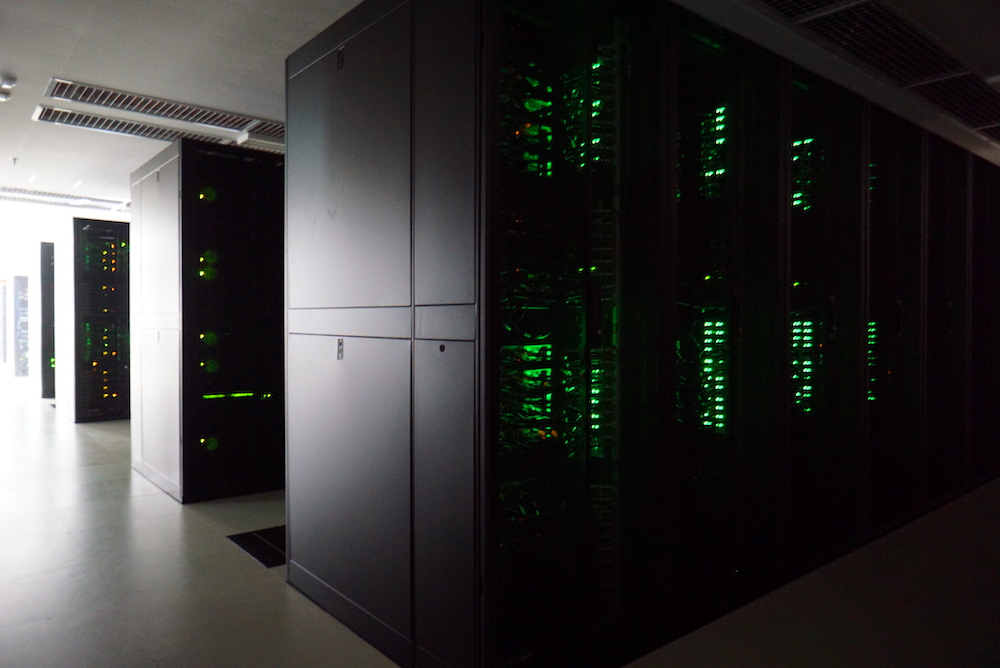
\includegraphics[width=.9\columnwidth]{figs/rack.jpg}
  \caption{AOBA-Sの外観}\label{fig:aoba-s}
\end{figure}

AOBA-Sは,表\ref{tbl:aoba-s}に示す通り
504ノードの日本電気社製SX-Aurora TSUBASA C401-8システムから構成されるスーパーコンピュータである.
図\ref{fig:node}にSX-Aurora TSUBASA (SX-AT) C401-8ノードの構成を示す.
SX-Aurora TSUBASAはVector Host (VH) とVector Engine (VE) の2種のプロセッサが搭載した
ヘテロジニアスな計算機である.VEはPCI Expressカード上に実装されたベクトルプロセッサであり,
アプリケーションの実行を担う.VEはHBMと密結合されており,特にメモリ律速のアプリケーションにおいて
高い性能を発揮する.VHはVEの制御を担い,VEから発行されたI/O等のOS処理を実行するx86\_64プロセッサである.
SX-AT C401-8はVHとして64コアのAMD EPYC 7763 CPUを採用しており,各ノードに8基のVector Engine Type
30Aカードを搭載している.8基のVEはPCIe Gen 4$\times$16によって
2基ずつ共有するPCIeスイッチを経由し,VHに接続している.
VEは1基あたり96\,GBのHBM2Eメモリ,VHは256\,GBのDDR4メモリを搭載している.また,VHには2基のInfiniBand
NDR200 HCAが搭載されており,VHおよびVE間で高速通信を実現している.

\begin{table}[tb]
\centering
\caption{AOBA-Sの性能諸元}\label{tbl:aoba-s}
\begin{tabular}{@{}lll@{}}
\toprule
ノード数        & ノード単体     & システム全体           \\ \midrule
VE数            & 8              & 4,032                  \\ \midrule
VH数            & 1              & 504                    \\
VE理論演算性能  & 39.28\,TFLOP/s & 19.79\,PFLOP/s         \\
VEメモリ帯域幅  & 19.60\,TB/s    & 9.87\,PB/s             \\
VEメモリ容量    & 768\,GB        & 378\,TB                \\ \midrule
VH理論演算性能  & 2.50\,TFLOP/s  & 1.26\,PFLOPS/s         \\
VHメモリ帯域幅  & 0.20\,TB/s     & 0.1\,PB/s              \\
VHメモリ容量    & 256\,GB        & 126\,TB                \\ \midrule
相互結合網      & \multicolumn{2}{c}{InfiniBand NDR}      \\
共有ストレージ  & \multicolumn{2}{c}{Lustre 4.4\,PB}      \\ \bottomrule
\end{tabular}
\end{table}

\begin{figure}[tb]
  \centering
  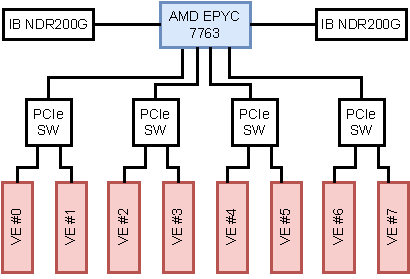
\includegraphics{figs/node_arch.pdf}
  \caption{SX-Aurora TSUBASA C401-8の構成}\label{fig:node}
\end{figure}

\subsection{Vector Engine Type 30A (VE30)}

\begin{figure}[tb]
  \centering
  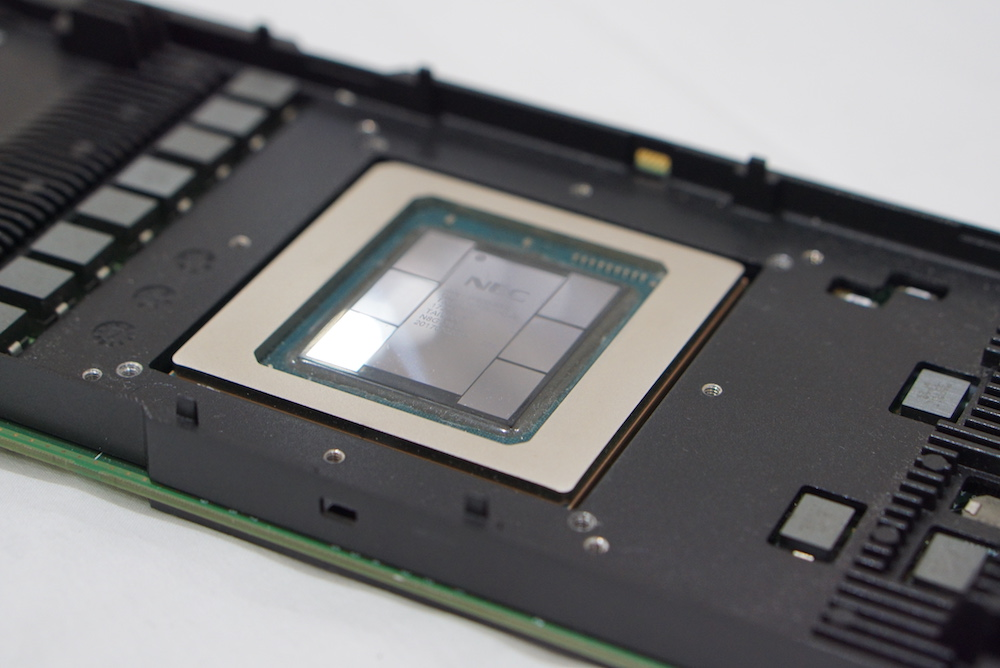
\includegraphics[width=.9\columnwidth]{figs/ve30.jpg}
  \caption{Vector Engine Type 30Aの外観}\label{fig:ve-card}
\end{figure}

図\ref{fig:ve30}にVector Engine Type 30A (VE30)プロセッサの概要を示す.VE30はVector
Engineプロセッサの第3世代となるプロセッサである.VE30は16個のベクトルコアを搭載し,これらの
ベクトルコアが2次元メッシュ型Network on Chip (NoC)によって接続されている.
ベクトルコア群はNoCによって6.4\,TB/sの帯域幅を有するLast Level Cache 
(LLC) に接続しており,さらにLLCは2.45\,TB/sの帯域幅を有する96\,GBのHBM2Eメモリに接続している.
各ベクトルコアはScalar Processing Unit (SPU) とVector Processing Unit (VPU) という2種の実行ユニット
を搭載している.SPUは命令をフェッチ,デコードし,VPUへベクトル命令を発行する.VPUはベクトル命令を
実行する.SPUにはL1キャッシュとL2キャッシュが搭載されており,さらに,VE30ではSPUとVPUが共有する
2\,MBのL3キャッシュが追加されている.

\begin{figure}[tb]
  \centering
  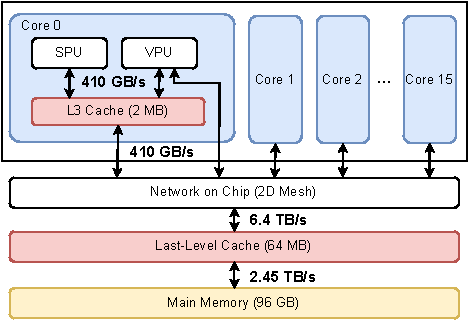
\includegraphics{figs/ve30_memory_hierarchy.pdf}
  \caption{VE30の概要図~\cite{Takahashi2023}}\label{fig:ve30}
\end{figure}

前世代のVE Type 20Aと比較すると,コアあたりの演算性能とメモリアクセス性能を同一である一方,
コア数が10コアから16コアへ1.6倍に増加し,プロセッサの演算性能は1.6倍に向上している.
また,コア数の増加に応じてメモリ帯域幅も1.53\,TB/sから
2.54\,TB/sへ1.6倍に向上している.さらに,メモリ容量は48\,GBから96\,GBへ2倍に拡大され,LLCの容量は
16\,MBから64\,MBへ4倍に拡大している.LLCの帯域幅は3.0\,TB/sから6.4\,TB/sに2.13倍に向上している.

\subsection{相互結合網とストレージ}

物理的には1ラックに16 VHが搭載されており,32ラックに計504 VHが収容されている.
これに加え,フロントエンドサーバ群および管理・監視サーバに2ラック,ネットワーク機器が2ラック,
UPSが3ラック,ストレージが1ラックの計8ラックに収容されている.

相互結合網にはInfiniBand NDRを採用しており,図\ref{fig:topo}に示すように,
フルバイセクション帯域幅およびノンブロッキングの2段Fat-treeトポロジによって計算ノード,
ストレージノード,およびフロントエンドノードが接続されている.相互結合網は16基のスパインスイッチおよび
18基のリーフスイッチによって構成される.各スイッチはNVIDIA Quantum-2 QM9700を採用している.
リーフスイッチのうち16基には計算ノードが接続されており,
残りの2基にはストレージおよび各種サーバ群が接続されている.計算ノードが接続されている
各リーフスイッチには32 VH (64 HCA) が接続されている.各スパインスイッチとリーフスイッチの間は2本の
400\,Gbpsリンクによって接続されており,計算ノード部分のバイセクション帯域幅は204.8\,Tbpsに達する.

\begin{figure}[tb]
  \centering
  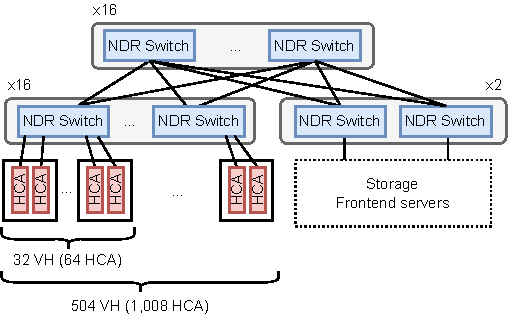
\includegraphics{figs/nw_topology.pdf}
  \caption{AOBA-Sの相互結合網}\label{fig:topo}
\end{figure}

ストレージには2基のDDN社製LustreアプライアンスであるES400NVX2を採用している.
1基のES400NVX2がMDS/MDT機能を提供しており,仮想マシンとして4台のMDSが稼働している.
MDTの実効容量は15.3\,TBであり,格納可能な最大i-node数は約55億である.
もう1基のES400NVX2はOSS/OST機能を提供しており,仮想マシンとして4台のOSSが稼働している.
OSS/OST用ES400NVX2には4基のSS9012エンクロージャが接続され,合計332本の7.2k\,rpm NL-SAS
HDDを搭載している.各ES400NVX2は8本のInfiniBand HDR100リンクによって相互結合網に接続している.
本ストレージは利用者毎の\verb|/uhome|領域として提供しているほか,
課題参加者間でファイルを共有するための\verb|/short|も提供している.
また,各ノードには1\,TBのSSDが搭載されており,高速一時領域\verb|/SSDTMP|として利用可能である.

\subsection{ソフトウェア環境}

利用者のプログラム開発環境として,高度な自動ベクトル化および自動並列化機能を備える
NEC C/C++コンパイラとFortranコンパイラを提供している.これらのコンパイラはそれぞれ
C++ 14/17とFortran 2008に準拠している.また,GNUツールチェーンの各種ツールがVE用に移植されており,
プロファイラとして\verb|ngprof|,デバッガとして\verb|ve-gdb|が利用可能である.さらに
プログラムの
ベクトル化率,平均ベクトル長,キャッシュヒット率等をハードウェアパフォーマンスカウンタによって
計測するためのツールとしてPROGINF,同様の情報を関数単位で計測するためのツールとしてFTRACEを
提供している.

数値計算ライブラリ集としてはNEC Numeric Library Collection
(NLC) を提供しており,BLAS,LAPACK,SBLAS,ScaLAPACK,FFTW互換のインターフェースを通じて
既存プログラムの移植を容易にしている.

\section{性能評価}

本節では,AOBA-Sのプロセッサよびシステム全体の多面的な性能評価結果について報告する.
まず,\ref{sec:proc}節においてVE30プロセッサの単体性能を報告し,\ref{sec:hpl-hpcg}節において
全系を用いたHPLおよびHPCGベンチマークの性能を報告する.
\ref{sec:mpi}節と\ref{sec:storage}節においてそれぞれMPI通信性能とストレージの性能について報告する.
最後に,\ref{sec:spechpc}節においてSPEChpcベンチマークスイート用いた実アプリケーションを想定した
性能評価を実施する.

\subsection{プロセッサ単体性能}\label{sec:proc}

VE30プロセッサの単体性能を同世代の他プロセッサと比較する.
比較対象のプロセッサは,前世代のVEであるVE Type 20B,富士通A64FX,Intel Xeon Platinum 8368
(IceLake),NVIDIA A100 PCIe 40\,GBおよび80\,GBモデルである.
各プロセッサの詳細な諸元については,文献~\cite{Takahashi2023}を参照されたい.

\subsubsection{基本性能}

まず,業界標準のベンチマークであるBabelStream~\cite{Deakin2018},
High Performance Linpack (HPL)~\cite{Dongarra2003},およびHigh Performance Conjugate
Gradients (HPCG)~\cite{Dongarra2016}を用いてVE30プロセッサの単体性能を同世代の他プロセッサと比較する.
HPLおよびHPCGのバイナリには,
各プロセッサのベンダより提供されている最適化されたバイナリを使用した.なおA64FXについてはバイナリを
入手できなかったため,Top500に掲載されている全系実行の性能より推定した.

図\ref{fig:stream}にBabelStream v4.0によって計測した各プロセッサの実効メモリ帯域幅を示す.
VE30の実効メモリ帯域幅は1.79\,TB/sとなり,他のすべてのプロセッサより高い性能となった.
一方,ピークメモリ帯域幅に対する効率は72\%であり,これはA100 40\,GBモデルの91\%や80\,GBモデルの
86\%に比べると低い.これは,VEのキャッシュラインサイズが128\,Bであるのに対し,GPUの
キャッシュラインサイズが256\,Bと2倍の大きさであるため,STREAMのような連続メモリアクセスにおいて
GPUが有利である可能性がある.

\begin{figure}[tb]
  \centering
  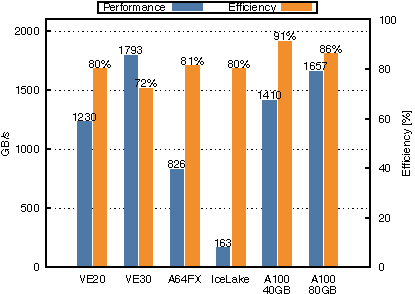
\includegraphics{figs/stream.pdf}
  \caption{BabelStream性能~\cite{Takahashi2023}}\label{fig:stream}
\end{figure}

図\ref{fig:hpl}にHPLベンチマークの性能を示す.HPLは演算律速なベンチマークであるため,ピーク演算性能が
高いA100 40\,GBモデルと80\,GBモデルの実効性能が11.8\,TFLOP/sと12.5\,TFLOP/sと非常に高い.
一方,実行効率は60\%台とVEやA64FXに比べると低い.
実行中に\verb|nvidia-smi|コマンドでGPUの周波数を監視すると周波数が低下しており,
PCIe版では電力供給が不足し,パワースロットリングによって性能低下していると考えられる.
VE30の性能は4.43\,TFLOP/sとなり,A100の両モデルに次いで最も高くなった.
実行効率は90\%と高く,\verb|vecmd|\footnote{\url{https://sxauroratsubasa.sakura.ne.jp/documents/guide/pdfs/InstallationGuide_E.pdf}}
コマンドで周波数を監視したところ,パワースロットリングは発生していなかった.よって,PCIeカードの
電力制約内で安定して性能を発揮できていると言える.

\begin{figure}[tb]
  \centering
  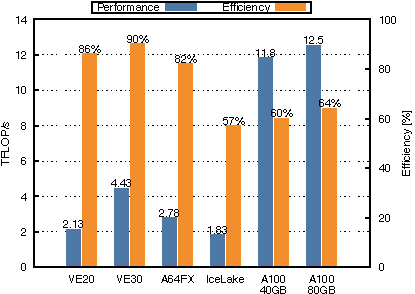
\includegraphics{figs/hpl.pdf}
  \caption{HPL性能~\cite{Takahashi2023}}\label{fig:hpl}
\end{figure}

図\ref{fig:hpcg}にHPCGベンチマークの性能を示す.VE30におけるHPCGベンチマークの性能は258\,GFLOP/sであり,
A100 80\,GBモデルの259\,GFLOP/sとほぼ同等の結果となった.実行効率は5.2\%であり,A100 80\,GBモデルの
2倍となった.

\begin{figure}[tb]
  \centering
  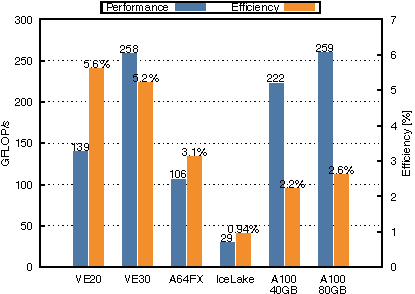
\includegraphics{figs/hpcg.pdf}
  \caption{HPCG性能~\cite{Takahashi2023}}\label{fig:hpcg}
\end{figure}

\subsubsection{東北大カーネル集}

実アプリケーションにおける性能を計測するため,本センターの利用者が開発した
アプリケーションから抽出したカーネルのカタログである東北大カーネル集の性能を測定した.
東北大カーネル集は,表\ref{tbl:isc-kernels}に示す6つのカーネルからなる.それぞれのカーネルは表に示す通り,
それぞれ律速要因が異なる.

\begin{table}[tb]
\caption{東北大カーネル集}\label{tbl:isc-kernels}
\begin{tabular}{@{}lll@{}}
\toprule
カーネル名                          & 科学分野        & 律速要因            \\ \midrule
Earthquake~\cite{Ariyoshi2007}      & 地震学          & メモリ帯域幅        \\
Turbulent Flow~\cite{Tsukahara2007} & 流体力学        & LLC帯域幅           \\
Antenna~\cite{Sato2011}             & 電波工学        & メモリ帯域幅        \\
Land Mine~\cite{Sato2003}           & 電波工学        & メモリ帯域幅        \\
Turbine~\cite{Tsukahara2007}        & 流体力学        & メモリレイテンシ    \\
Plasma~\cite{Katoh2005}             & プラズマ科学    & メモリレイテンシ    \\ \bottomrule
\end{tabular}
\end{table}

図\ref{fig:isc-kernels}にVE20およびVE30における東北大カーネル集の性能を示す.VE30では,新設された
L3キャッシュの効果を明らかにするため,L3キャッシュをバイパスした際の性能も合わせて示している.
まず,メモリ帯域幅に律速されるEarthquake, Antenna, Land MineではVE30はVE20に比べ1.6倍高速化しており,
これはメモリ帯域幅の向上率と一致している.LLC帯域幅律速であるTurbulent Flowでは,2.26倍高速化
してり,同じくLLC帯域幅の向上率2.13倍とほぼ一致している.
メモリレイテンシ律速であるTurbineとPlasmaではそれぞれ2.39倍と2.42倍性能が向上しており,メモリ帯域幅
やLLC帯域幅のいずれの向上率も超えている.
これは新設されたL3キャッシュにヒットすることにより,メモリレイテンシが短縮していることに起因する.

\begin{figure}[tb]
  \centering
  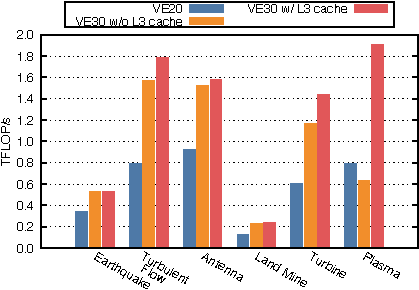
\includegraphics{figs/isc_kernels.pdf}
  \caption{東北大カーネル集の性能}\label{fig:isc-kernels}
\end{figure}

% Earthquake	1.562433029	1.562414022
% Turbulent Flow	2.269235107	1.987005372
% Antenna	1.713382084	1.649130386
% Land Mine	1.840124773	1.815984976
% Turbine	2.39612046	1.941414462
% Plasma	2.424101774	0.801012457

\subsection{HPL・HPCG性能}\label{sec:hpl-hpcg}

HPLベンチマークおよびHPCGベンチマークを複数VH上で実行し,性能を計測した.
504 VHを用いた全系実行では,HPL性能が16.33\,PFLOP/s (実行効率82.4\%),HPCG性能が913.1\,TFLOP/s 
(実行効率4.61\%) となった.
なお,これらの性能はパラメータのチューニング等の最適化を未実施の状態での性能であるため,
今後チューニングを実施することにより,さらに性能が向上する予定である.

\begin{figure}[tb]
  \centering
  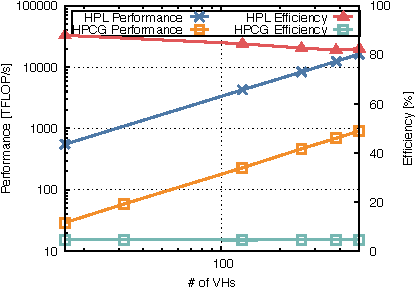
\includegraphics{figs/hpl_hpcg.pdf}
  \caption{HPLおよびHPCG性能}\label{fig:hpl-hpcg}
\end{figure}

\subsection{MPI通信性能}\label{sec:mpi}

OSU Micro-Benchmarks
7.2\footnote{\url{https://mvapich.cse.ohio-state.edu/benchmarks/}}を用いてMPI通信の性能を計測した.
測定にあたっては,(1) 同一PCIeスイッチ配下のVE間,(2)
同一VH内の異なるPCIeスイッチ配下のVE間,(3) 同一ラックの異なるVH配下のVE間,
(4) 同一ラックの異なるVH間,の4パターンを計測した.
ベンチマークを実行する際には\verb|-i 1000 -x 500|オプションを指定し,
繰り返し回数を1,0000回,ウォームアップ回数を500回にそれぞれ設定した.
MPIライブラリには,NECが提供するNEC MPI 3.4.0を用いた.

図\ref{fig:mpi-lat}に\verb|osu_latency|ベンチマークで計測したMPI 1対1通信のレイテンシを示す.
同一PCIeスイッチ配下のVE間における最低レイテンシは1.51$\mu$sであった.
同一VH内の異なるPCIeスイッチ配下のVE間ではルートコンプレックスを経由する必要があるため,レイテンシが
増加し,1.88$\mu$sとなった.同一ラックの異なるVH配下のVE間のレイテンシは3.87$\mu$sであった.
これらのVE間のレイテンシは,GPU-awareなMPI実装\cite{Shafie2021,Shafie2022}と同等の値である.
同一ラックの異なるVH間のレイテンシは2.09$\mu$sであった.

\begin{figure}[tb]
  \centering
  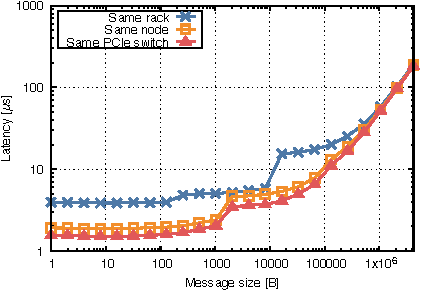
\includegraphics{figs/mpi_latency.pdf}
  \caption{MPI 1対1通信のレイテンシ}\label{fig:mpi-lat}
\end{figure}

\begin{figure}[tb]
  \centering
  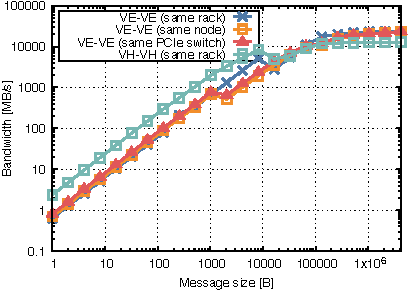
\includegraphics{figs/mpi_bandwidth.pdf}
  \caption{MPI 1対1通信のスループット}\label{fig:bw}
\end{figure}

図\ref{fig:mpi-lat}に\verb|osu_bandwidth|ベンチマークで計測したMPI 1対1通信のスループットを示す.
スループットではVE間の通信経路によって大きな差が見られず,
同一PCIeスイッチ配下のVE間で23.1\,GB/s,同一VH内の異なるPCIeスイッチ配下のVE間で22.7\,GB/s,
同一ラックの異なるVH配下のVE間で 23.6\,GB/sであった.
InfiniBanad NDR200の理論帯域幅は25\,GB/sであるため,VHを跨ぐVE間通信のスループットは
94\%と高い効率を達成している.一方,VH内のVE間通信ではPCIeリンク帯域幅が律速要因となるはずだが,
PCIe Gen 4 $\times$16の理論帯域幅31.5\,GB/sに対して73\%程度の効率に留まっている.
VH間のスループットは22.8\,GB/sとなり,VE間のスループットと同程度であったものの,
32\,KiB以下のメッセージサイズではVH間のスループットがVE間に比べ3倍程度高かった.
これはVHとVEのプロセッサの性能差に起因すると考えられる.

\subsection{ストレージ性能}\label{sec:storage}

IOR 3.3.0\footnote{\url{https://github.com/hpc/ior}}を用いて並列ファイルシステムのスループットを計測した.
1 VEにつきIORを1プロセスを起動し,プロセスごとに別ファイルに書き込む設定で計測を実施した.
計測に用いたコマンドは,
\texttt{ior -w -r -a POSIX -F -Q 8 -C -e -g -b 16m -t 4m -s 250 -i 3}である.
書き込み時のページキャッシュの効果を排除するため,\texttt{-e}オプションによってwrite完了時に
\texttt{fsync()}を呼び出している.また,読み込み時のページキャッシュの効果を排除するため,書き込み
プロセスと読み込みプロセスをずらす\texttt{-C}オプションを指定している.同一VHに接続された
VEはVH側においてページキャッシュを共有するため,書き込みプロセスと読み込みプロセスがそれぞれ異なるVH
配下のVE上で動作するよう,
\texttt{-Q 8}オプションによって書き込みと読み込みプロセスを8ランク分ずらしている.

図\ref{fig:ior}に計測結果を示す.1,024プロセスにおいて書き込み49.2\,GB/s,読み込み39.0\,GB/sの
スループットを達成した.

\begin{figure}[tb]
  \centering
  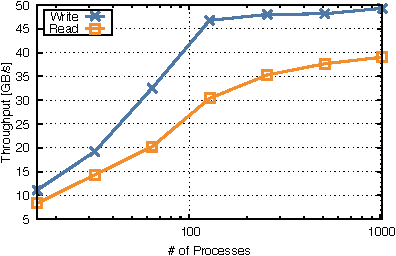
\includegraphics{figs/ior.pdf}
  \caption{並列ファイルシステムの読み書き性能}\label{fig:ior}
\end{figure}

また,図\ref{fig:mdtest}にIORに付属するMDTESTを用いて計測した並列ファイルシステムのメタデータ性能を
示す.メタデータ性能は512プロセス程度でピークに達し,File statの性能が189\,KIOpsとなった.

\begin{figure}[tb]
  \centering
  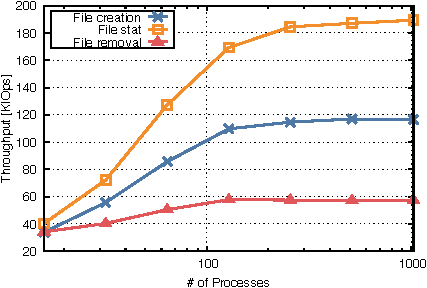
\includegraphics{figs/mdtest.pdf}
  \caption{並列ファイルシステムのメタデータ性能}\label{fig:mdtest}
\end{figure}

\subsection{SPEChpc}\label{sec:spechpc}

SPEChpc 2021\cite{Li2022,Kodama2023}は,Standard Performance Evaluation Corporation (SPEC) が開発する
HPC向けのベンチマーク集である.SPEChpc 2021はTiny,Small,Medium,Largeの問題サイズが異なる
4種のベンチマークスイートを提供しており,TinyとSmallスイートが9つ,MediumとLargeスイートが6つの
ベンチマークからなる.各ベンチマークの性能値はベースラインシステム (独TU Dresdenに設置されているTaurus) 
に対する高速化率として報告される.
全てのベンチマークは,フラットMPI,MPI+OpenMP,MPI+OpenACC,MPI+OpenMP Target Offloadingの
4種のプログラミングモデルを利用可能である.本評価ではVEおよびCPUではMPI+OpenMP,GPUではMPI+OpenACCを
使用する.

本評価では,2022年7月にリリースされたSPEChpc 2021 V1.1.7を使用する.VE30でベンチマークをコンパイル
する際のコンパイラオプションには,\texttt{-O4 -finline-functions}を使用する.
また,ベクトル化率およびベクトル長を向上させるため,
LBMには \texttt{-mretain-none -fivdep -floop-unroll-complete=37},
POT3DとminiWeatherには \texttt{-fivdep-omp-worksharing-loop}を指定する.
SPEChpcの実行ルールでは,OpenMPまたはOpenACC指示行を除いて,一切のソースコードの変更を許していない.
したがって,本評価ではソースコードを一切修正せず実行する.

\begin{figure*}[tb]
  \centering
  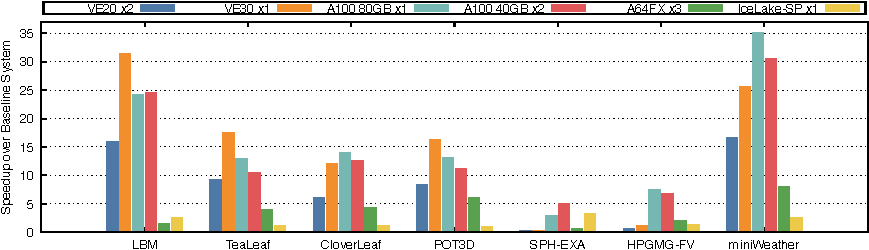
\includegraphics{figs/spechpc_tiny.pdf}
  \caption{SPEChpc Tinyスイートの性能}\label{fig:spechpc-t}
\end{figure*}

\subsubsection{Tinyサイズ}

Tinyサイズは実行に約60\,GBのメモリを要し,主として単一ノードでの実行を想定している.
メモリ容量が不足するプロセッサについては,実行可能な最小ソケット数で実行し,高速化率を使用
ソケット数で正規化して報告する.なおTinyスイートのベンチマークのうち
SOMAとMinisweepはコンパイラの不具合のため結果不整合が発生したため,これらのベンチマークは除いて
報告する.

図\ref{fig:spechpc-t}にTinyスイートの性能比較を示す.VE30はLBM,TeaLeaf,POT3Dの3つのベンチマークにおいて
他のすべてのプロセッサを上回る性能を達成している.これらのベンチマークにおけるA100 80\,GBに対する
性能差はそれぞれ1.29$\times$,1.36$\times$,1.24$\times$である.LBMとTeaLeafの性能差は
VE30とA100のメモリ帯域幅の差を超えており,新設されたL3キャッシュや拡張されたLLCが性能に寄与している
ことがわかる.

また,VE30の性能ははA64FXとIceLake-SPをCloverLeafとminiWeatherにおいて上回るものの,
A100 40\,GBと80\,GBをやや下回る.これは,CloverLeafのカーネルはギャザメモリアクセスを要求するが,
A100がギャザのレイテンシの隠蔽においてVE30より優れるためと考えられる.また,miniWeatherは
メモリ律速のカーネルと演算律速のカーネルの両方を含み,メモリ律速のカーネルはVE30がA100より
高性能なものの,演算律速のカーネルのA100に劣るため,全体としてはA100に性能が劣っている.

SPH-EXAとHPGMG-FVのVE30における性能は低い.SPH-EXAは粒子法の一種である
Smoothed Particle Hydrodynamics (SPH) 法に基づくベンチマークであり,8分木を用いた近傍粒子探索を
行う.8分木の構築と探索はいずれも再帰呼び出しを用いて実装されており,ベクトル化ができないため,VE30
において性能が非常に低く,ボトルネックとなっている.
ベクトルプロセッサでは性能を向上するためには,近傍粒子探索をベクトル化可能なアルゴリズム
に変更する必要がある.

HPGMG-FVは平均ベクトル長の短さによって性能が低くなっている.Tinyスイートにおいては,
$512^3$の格子を$32^3$の格子に領域分割し,各部分格子をMPIランクに分散している.
ボトルネックとなる赤-黒順序付けGauss-Seidelスムーザは長さ32の3重ループとなるが,
しかし,倍精度で256要素保持できるVEのベクトルレジスタに対してはループ長が短すぎるため,
効率が低くなっている.性能を向上するには,loop collapseによるループ長の拡大が考えられる.
また,粗い格子レベルをホスト側で実行する最適化も考えられる.

\subsubsection{Largeサイズ}

\begin{figure}[tb]
  \centering
  \begin{minipage}[b]{0.46\hsize}
    \centering
    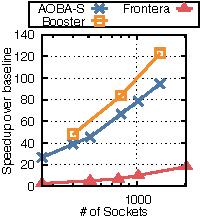
\includegraphics{figs/spechpc_lbm_l.pdf}
    \subcaption{LBM}\label{fig:lbm-l}
  \end{minipage}
  \begin{minipage}[b]{0.46\hsize}
    \centering
    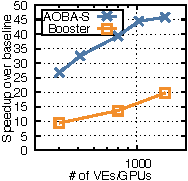
\includegraphics{figs/spechpc_tealeaf_l.pdf}
    \subcaption{TeaLeaf}\label{fig:tealeaf-l}
  \end{minipage} \\
  \begin{minipage}[b]{0.46\hsize}
    \centering
    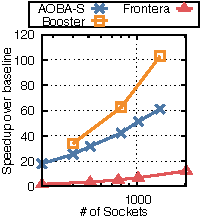
\includegraphics{figs/spechpc_clvleaf_l.pdf}
    \subcaption{CloverLeaf}\label{fig:clvleaf-l}
  \end{minipage}
  \begin{minipage}[b]{0.46\hsize}
    \centering
    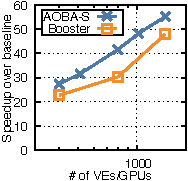
\includegraphics{figs/spechpc_pot3d_l.pdf}
    \subcaption{POT3D}\label{fig:pot3d-l}
  \end{minipage} \\
  \begin{minipage}[b]{0.46\hsize}
    \centering
    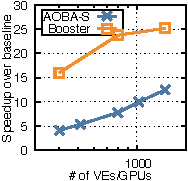
\includegraphics{figs/spechpc_hpgmgfv_l.pdf}
    \subcaption{HPGMG-FV}\label{fig:hpgmg-l}
  \end{minipage}
  \begin{minipage}[b]{0.46\hsize}
    \centering
    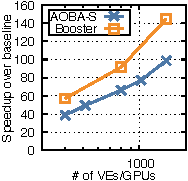
\includegraphics{figs/spechpc_weather_l.pdf}
    \subcaption{miniWeather}\label{fig:weather-l}
  \end{minipage}
  \caption{SPEChpc Largeスイートの性能}\label{fig:spechpc-l}
\end{figure}

Largeサイズは約14.5\,TBのメモリを必要とし,大規模なクラスタを対象としている.
本報告の執筆時点ではAOBA-S以外の大規模実行環境を準備することができなかったため,
ここでは文献~\cite{Brunst2022}において計測が
なされた,米Texas Advanced Computing CenterのFronteraおよび独J\"{u}lich Supercomputing Centreの
JUWELS Booster上での性能測定結果を参照する.FronteraはノードあたりIntel Xeon Platinum 8280を2
ソケット搭載し,InfiniBand HDR100を1ポート備えるシステムである.
BoosterはノードあたりAMD EPYC 7402を2ソケットとNVIDIA A100 SXM4 40\,GBを4基搭載し,
InfiniBand HDR200を4ポート備えるシステムである.

図\ref{fig:spechpc-l}にLargeスイートの性能を示す.
全体の問題サイズは$4096^3$に増大しているものの,1ランクに配布される部分格子のサイズは$2^5$のまま
であり,ベクトル長の短さが性能劣化の要因となっている.
LBM,CloverLeaf,miniWeatherでは特にプロセス数数が増加するとBoosterとの性能差が拡大することから,
Boosterに比べスケーラビリティが劣っている.この原因として,(1) 通信性能の差 (2)
プログラム起動時間の差,の2点を仮説として,検証を試みた.

まずNEC MPI\footnote{\url{https://sxauroratsubasa.sakura.ne.jp/documents/mpi/pdfs/g2am01-NEC_MPI_User_Guide_ja.pdf}}のプロファイラ機能を用いて,各ベンチマークの実行時間に占めるMPI通信時間を計測した.
図\ref{fig:spechpc-profile1}にプロファイル結果を示す.
LBMとCloverLeafでは5\%程度,miniWeatherでは20\%と,通信時間の占める割合は多くない.したがって,
MPI通信性能がスケーラビリティを制限しているとは考えられない.

\begin{figure}[tb]
  \centering
  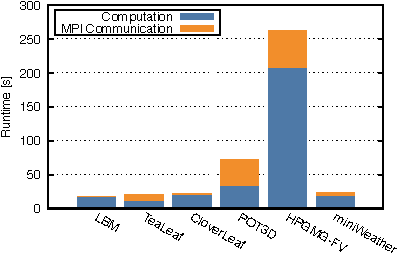
\includegraphics{figs/spechpc_profile.pdf}
  \caption{SPEChpc Largeサイズの実行時間内訳}\label{fig:spechpc-profile1}
\end{figure}

次に,SPEChpcプログラム起動時間の差を検証する.SPEChpcでは,
mpirunを呼び出してから終了するまでの時間をベンチマークの実行時間としている.大規模実行では
MPIプログラムの起動に係る時間が無視できないため,プログラム起動時間を計測した.
具体的には,SPEChpc
V1.1より導入された内蔵タイマ\footnote{\url{https://www.spec.org/hpc2021/Docs/changes-in-v1.1.html#timer}}を利用し,ベンチマークごとに次の時間を計測した:

\begin{description}
  \item[Launch Overhead Time] ノード,スケジューラ,MPIの起動に費やされた時間
  \item[Application Init Time] データの初期化,ファイル読み込み,領域分割等の初期化処理に費やされた時間
  \item[Application Core Time] プログラムの主たる計算処理に費やされた時間
  \item[Application Resid Time] 計算結果の検証や計算結果の出力等,Init TimeおよびCore Time以外の処理
      に費やされた時間
\end{description}

図\ref{fig:spechpc-profile2}に各ベンチマークの実行時間の内訳を示す.
まず,Application Init TimeとResidual Timeは全てのベンチマークにおいて無視可能であった.一方,
Launch Overhead Timeはベンチマークに関わらず常に10秒以上であり,特に計算時間が短い
LBM,TeaLeaf,CloverLeaf,miniWeatherでは実行時間の1/3以上と大きな割合を占める.
BoosterおよびFronteraの性能値を参照した文献~\cite{Brunst2022}では,このような実行時間の内訳を
公開していないため,現時点では他システムにおけるLaunch Overhead
Timeは不明だが,性能差の一因となっている可能性がある.今後は,AOBA-Sにおける起動時間を短縮できるか
検討するほか,他システムにおいて大規模実行を実施し,Launch Overhead Timeの計測を目指す.

\begin{figure}[tb]
  \centering
  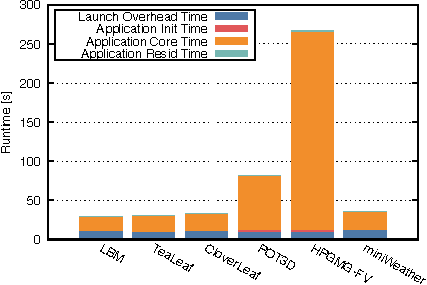
\includegraphics{figs/spechpc_profile2.pdf}
  \caption{SPEChpc Largeサイズの実行時間内訳}\label{fig:spechpc-profile2}
\end{figure}

\section{おわりに}

本稿では東北大学サイバーサイエンスセンターにおいて2023年8月ようり稼働開始したAOBA-Sの設計を示し,
運用開始に先駆けて実施した性能評価の結果を報告した.AOBA-Sは第3世代Vector Engine
プロセッサを採用したベクトル型スーパーコンピュータであり,メモリ律速のアプリケーションにおいて
同世代のCPUおよびGPUと同等以上の優れた性能を発揮できることが示された.一方,大規模な実行においては
他システムよりスケーラビリティが劣る場合が存在することが明らかになったので,今後は
さらに性能評価および性能分析を進め,得られた知見を利用者に還元していく.

\subsection*{謝辞}

性能評価にご協力いただいた東北大学情報部デジタルサービス支援課および日本電気株式会社の皆様に
感謝いたします.
本研究成果の一部は,大阪大学サイバーメディアセンターの「SQUID」および
名古屋大学情報基盤センターの「不老」を利用して得られたものです.

\bibliographystyle{IEEEtran}
\bibliography{references}

\end{document}
